\documentclass[correction]{exercices}
\usepackage{ae, aeguill, graphicx}
\usepackage{fullpage}
\usepackage{xspace}
\usepackage{color}
\usepackage{amsmath, amssymb}
\usepackage{latexsym}
\usepackage{url}
\usepackage{tikz}
\usetikzlibrary{trees,chains,positioning}
\usepackage{verbatim}
\renewcommand{\labelenumi}{(\alph{enumi})}

\usepackage{multicol}
\usepackage{listings}
\usepackage{verbatim}

\lstset{language=java, showstringspaces=false}


\begin{document}

\sujet{Exercices 2009: Exam 2008 + Sorting exercice}

\section{Multiple choice questions (9 points)}

  There is only \textbf{one} correct answer per question, the grading is :

  \begin{tabular}{rl}
  $1$    &point for a correct answer.\\
  $-0.5$ &points for a wrong answer.\\
  $0$    &points for a unanswered question.\\
  \end{tabular}
\vspace{1cm}

\begin{question}
A \textbf{final} method
\begin{multicols}{2}
\begin{enumerate}
\item cannot be invoked
\correct{cannot be overriden}
\item must be overriden
\item must be static
\end{enumerate}
\end{multicols}
\end{question}

\begin{question}
Which one of these propositions is \textbf{true} ?
\begin{enumerate}
\item The method main can be declared protected.
\correct{A private method can only be called from inside its own class.}
\item A method with no modifier can be called from a subclass.
\item Private methods cannot be static.
\end{enumerate}
\end{question}

\begin{question}
Which one of these propositions is \textbf{false} ?
\begin{enumerate}
\correct{A subclass of an abstract class must be concrete.}
\item An abstract class can implement an interface.
\item An abstract class can have static methods.
\item An abstract class can have final methods.
\end{enumerate}
\end{question}

\begin{question}
Which one of these propositions is \textbf{false} ?
\begin{enumerate}
\item An interface can extend another interface.
\correct{An interface can provide bodies for some of its methods.}
\item A class can implement more than one interface.
\item An interface can be used as a type.
\end{enumerate}
\end{question}

\begin{question}
\hfill

\begin{verbatim}
class A {
  void foo() {System.out.print("A");}
}
class B extends A {
  void foo() {System.out.print("B");}
}
class C {
  public static void main(String args[]) {
    A a = new A();
    B b = new B();
    A c = b;
    a.foo();
    b.foo();
    c.foo();
  }
}
\end{verbatim}

What is printed when we run class C ?
\begin{multicols}{2}
\begin{enumerate}
\item nothing because it produces an error
\correct{ABB}
\item ABA
\item AAA
\end{enumerate}
\end{multicols}
\end{question}


\begin{question}
\hfill

\begin{verbatim}
class A {
  A () {System.out.print("A");}
  A (int i) {System.out.print("A" + i);}
}
class B extends A {
  B (int i) {System.out.print("B" + i);}
}
class C extends B {
  C (int i) {super(i);i++;System.out.print("C"+i);}
  C () {this(1);}
}
\end{verbatim}

What is printed when we call \lstinline!new C();! ?
\begin{multicols}{2}
\begin{enumerate}
\item B1AC2
\item A1B1C2
\item B1C2A
\correct{AB1C2}
\end{enumerate}
\end{multicols}
\end{question}

\begin{question} \hfill
\begin{verbatim}
public class A {
  static void foo(int i, String[] st) {
    i--;
    st[i] = "bye";
  }
  public static void main(String args[]) {
    int i = 1;
    String greetings[] = {"hello","bye"};
    foo(i,greetings);
    System.out.println(greetings[0] + greetings[1] + i);
  }
}
\end{verbatim}

What does this program prints ?
\begin{multicols}{2}
\begin{enumerate}
\correct{byebye1}
\item byebye0
\item hellohello1
\item nothing because it produces an error
\end{enumerate}
\end{multicols}
\end{question}

\begin{question} \hfill
\begin{verbatim}
public class A {
  void bar() throws Exception {
    System.out.println("A");
    throw new Exception();
  }
  void foo() {
    try {
      System.out.println("C");
      bar();
      System.out.println("D");
    } catch (Exception e) {
      System.out.println("E");
      throw e;
    }
  }
  public static void main(String args[]) {
    A a = new A();
    a.foo();
  }
}
\end{verbatim}

What does this program prints ?
\begin{multicols}{2}
\begin{enumerate}
\item CAE
\item CADE
\item CAD
\correct{nothing because it does not compile}
\end{enumerate}
\end{multicols}
\end{question}

\begin{question} \hfill
\begin{verbatim}
String a = "hello";
String b = "hell";
String c = b + "o";
String d = a ;
\end{verbatim}

Which one of these propositions is \textbf{true} ?

\begin{multicols}{2}
\begin{enumerate}
\item a == c
\correct{a.equals(c)};
\item d == c;
\item c == d;
\end{enumerate}
\end{multicols}
\end{question}

\pagebreak
\section{Tree operations (7 points)}

The class below models a binary tree.
A binary tree is composed of nodes.
Each node has either two children or none at all.
A node without childrens is called a \textbf{leaf}.

Read and understand this class,  here is a drawing of the
Tree T that is constructed in main:
\begin{figure}[h]
\begin{tikzpicture}
  \node at(0,0) {0}
    child{node{5}}
    child{node{4}
      child{node{1}}
      child{node{2}}};
\end{tikzpicture}
\end{figure}

\begin{verbatim}
class Tree {
  int nodeValue;
  boolean leaf;
  Tree left;
  Tree right;

  Tree(int nodeValue) {
    this.nodeValue = nodeValue;
    leaf = true;
  }

  Tree(int nodeValue, Tree left, Tree right) {
    this.nodeValue = nodeValue;
    this.left = left;
    this.right = right;
    leaf = false;
  }

  int getSum() {...}
  boolean contains(int value) {...}

  public static void main(String args[]) {
    Tree T = new Tree(0, new Tree(5), new Tree(4, new Tree(1), new Tree(2)));
    System.out.println("Sum of all the nodeValues = " + T.getSum());
    System.out.println("Is value 5 in the tree ? " + T.contains(5));
  }
}
\end{verbatim}

\begin{question} (\textbf{3.5 points})\\
Implement the body of method \lstinline!int getSum()!.
This method should return the sum of all the node values of the calling tree.
(For T it would be $12$).

\begin{correction}
\begin{verbatim}
int getSum() {
    if (leaf)
      return nodeValue;
    else
      return nodeValue + left.getSum() + right.getSum();
  }
\end{verbatim}
\end{correction}
\end{question}

\begin{question} (\textbf{3.5 points}) \\
Implement the body of method \lstinline!boolean contains(int value)!.
This method returns \lstinline!true! if and only if value is equal to one
of the nodeValues in the tree.

\begin{correction}
\begin{verbatim}
  boolean contains(int value) {
    if (leaf)
      return nodeValue == value;
    else
      return left.contains(value) || right.contains(value);
  }
\end{verbatim}
\end{correction}
\end{question}

\section{Summing vectors (4 points)}

The class Vector belows models a vector of integer values.

Complete methods length and sumWith.

Method length should return the number of elements in the current vector.

Method sumWith should compute the sum element by element of the current
vector with another one, keeping the results in the current one.
Method sumWith should throw NotTheSameLength exception if vectors are of
different size.

\begin{verbatim}
class NotTheSameLength extends Exception {}
class Vector {
  int [] values;
  Vector(int [] values) {this.values = values;}
  int length(){...}
  void sumWith(Vector anotherVector) throws NotTheSameLength {...}

  public static void main(String args[]) {
    try {
      Vector V1 = new Vector(new int[]{1,2,3,4,5});
      Vector V2 = new Vector(new int[]{6,4,2,8,1});
      V1.sumWith(V2);
      /* here V1 values should be {7, 6, 5, 12, 6} */
    }
    catch (NotTheSameLength e) {
      System.out.println("Vectors must have the same length!");
    }
  }
}
\end{verbatim}


\begin{correction}
\begin{verbatim}
  int length(){return this.values.length;}

  void sumWith(Vector anotherVector) throws NotTheSameLength
  {
    if (this.length() != anotherVector.length()) throw new NotTheSameLength();
    for (int i=0;i<this.length();i++) {
      this.values[i] += anotherVector.values[i];
    }
  }
\end{verbatim}
\end{correction}

\pagebreak
\section{QuickSort :  extra exercice, not in the original exam}

The QuickSort algorithm, sorts a collection of elements with
a mean complexity of $O(nlog(n))$. In this exercice you are going to
use it to sort a list of strings. Below we explain the algorithm
(without loss of generality we use integers instead of strings):
\begin{enumerate}
\item Start with a list of elements.
  If the list is composed of only one element, or is empty stop.\\
  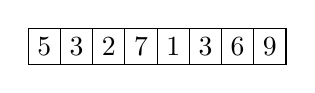
\begin{tikzpicture}[start chain=1 going right,node distance=-0.15mm]
    \foreach \x in {5,3,2,7,1,3,6,9} {
      \node [draw,on chain=1] {\x};
    }
  \end{tikzpicture}
\item Choose the first element as pivot.\\
  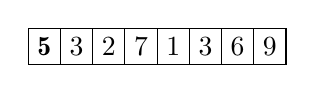
\begin{tikzpicture}[start chain=1 going right,node distance=-0.15mm]
    \node [draw,on chain=1] {\textbf{5}};
    \foreach \x in {3,2,7,1,3,6,9} {
      \node [draw,on chain=1] {\x};
    }
  \end{tikzpicture}
\item Move to the beginning of the list all the elements equal or smaller than pivot, and move to the end of the list  all the elements larger:\\
  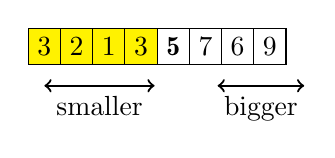
\begin{tikzpicture}[start chain=1 going right,node distance=-0.15mm]
    \foreach \x in {3,2,1,3} {
      \node [draw,on chain=1, fill=yellow] {\x};
    }
    \node [draw,on chain=1] {\textbf{5}};
    \foreach \x in {7,6,9} {
      \node [draw,on chain=1] {\x};
    }
    \path[draw,<->,thick] (0,-0.5) -- (1.4,-0.5) node[anchor=north,pos=0.5]
    {smaller};
    \path[draw,<->,thick] (2.2,-0.5) -- (3.3,-0.5) node[anchor=north,pos=0.5] {bigger};
  \end{tikzpicture}
\item Apply this same procedure ((a) to (d)) recursively on ``smaller''
  and ``bigger'' part of the list.
\end{enumerate}


You are going to implement the above algorithm on an array of
Strings, to achieve this you must provide the missing bodies
in the following java program.
\begin{verbatim}
public class QSort {
  static void qsort(String l[], int from, int to) {}
  static int partition(String l[],int from,int to) {}
  static void exch(String l[], int i, int j) {}

  public static void main(String args []){
    qsort(args, 0, args.length-1);
    for (int i = 0; i < args.length; i++) {
      System.out.println(args[i]);
    }
  }
}
\end{verbatim}

\begin{question}
Implement method \verb!exch!, which exchanges
in array \verb!l! the elements at positions \verb!i! and \verb!j!.
\end{question}
\begin{question}
Using \verb!exch! implement method \verb!partition! which should do the steps (b)
and (c) of the algorithm on the elements between position \verb!from!
and position \verb!to! (the extremas are included), it should return
the position of the chosen pivot.

That is to say, method \verb!partition! should choose a pivot between
position \verb!from! and position \verb!to!. And reorganize the elements
between position \verb!from! and position \verb!to! using \verb!exch!
so that all the elements smaller than pivot are at the beginning.
\end{question}
\begin{question}
Using method \verb!partition!,
implement the method \verb!qsort!,
that should sort the elements between position \verb!from!
and position \verb!to! in the list \verb!l!.
\end{question}

\end{document}
